\chapter{硬件信息表}%
\section{中断向量表}
\label{sec:zdxlb}
\begin{figure}[H]
  \centering
  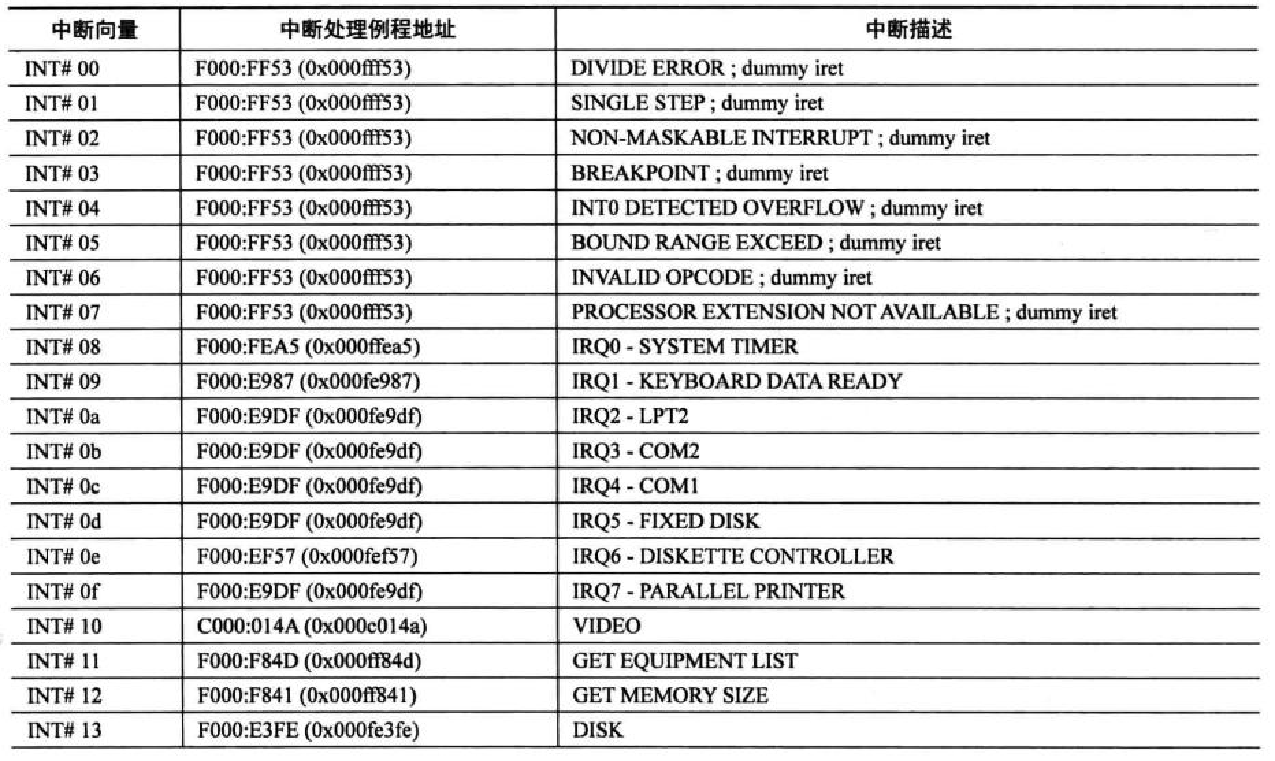
\includegraphics[width=15cm]{中断1}
  \caption{中断向量表1}
  \label{fig:itpt1}
\end{figure}
\begin{figure}[H]
  \centering
  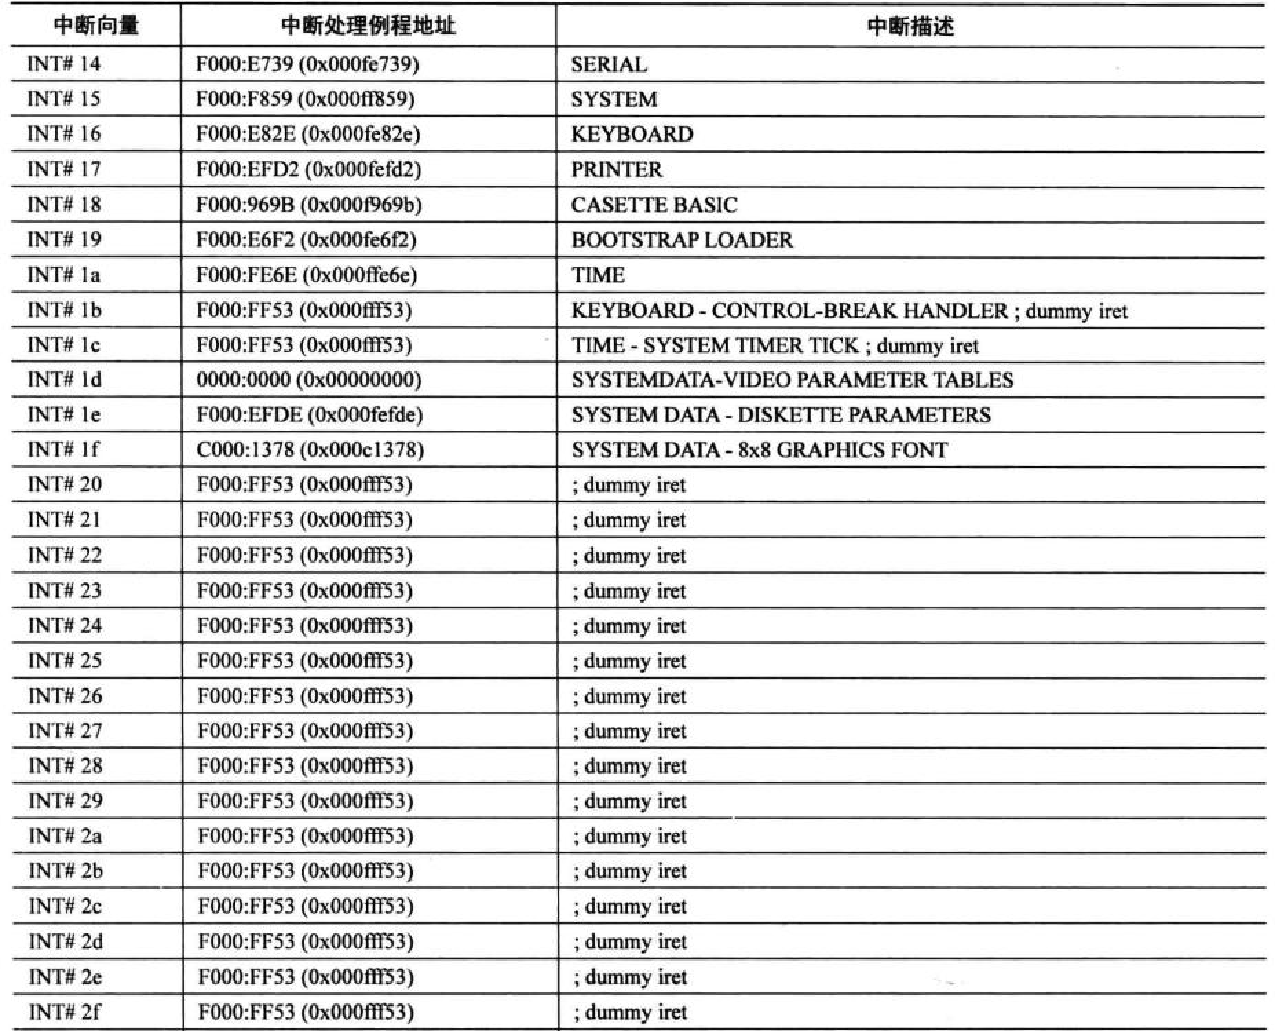
\includegraphics[width=15cm]{中断2}
  \caption{中断向量表2}
  \label{fig:itpt2}
\end{figure}
\begin{figure}[H]
  \centering
  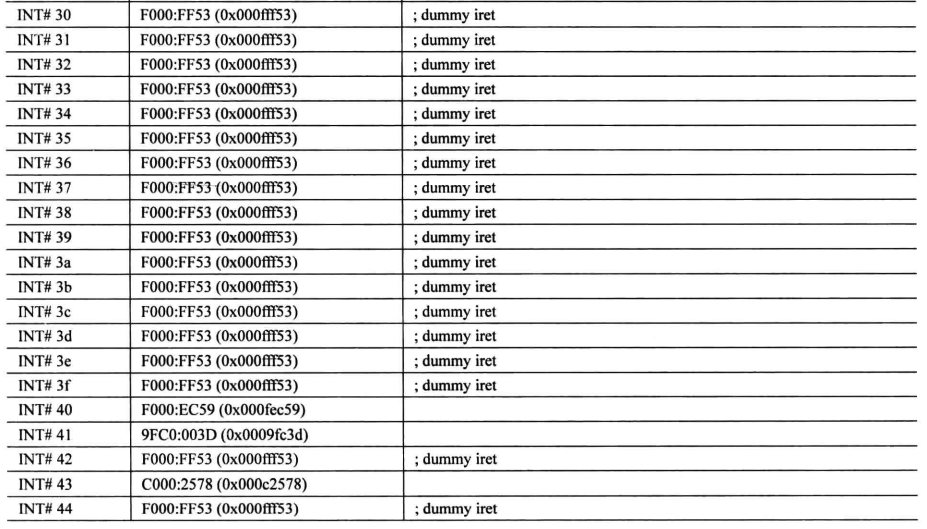
\includegraphics[width=15cm]{中断3}
  \caption{中断向量表3}
  \label{fig:itpt3}
\end{figure}
\begin{figure}[H]
  \centering
  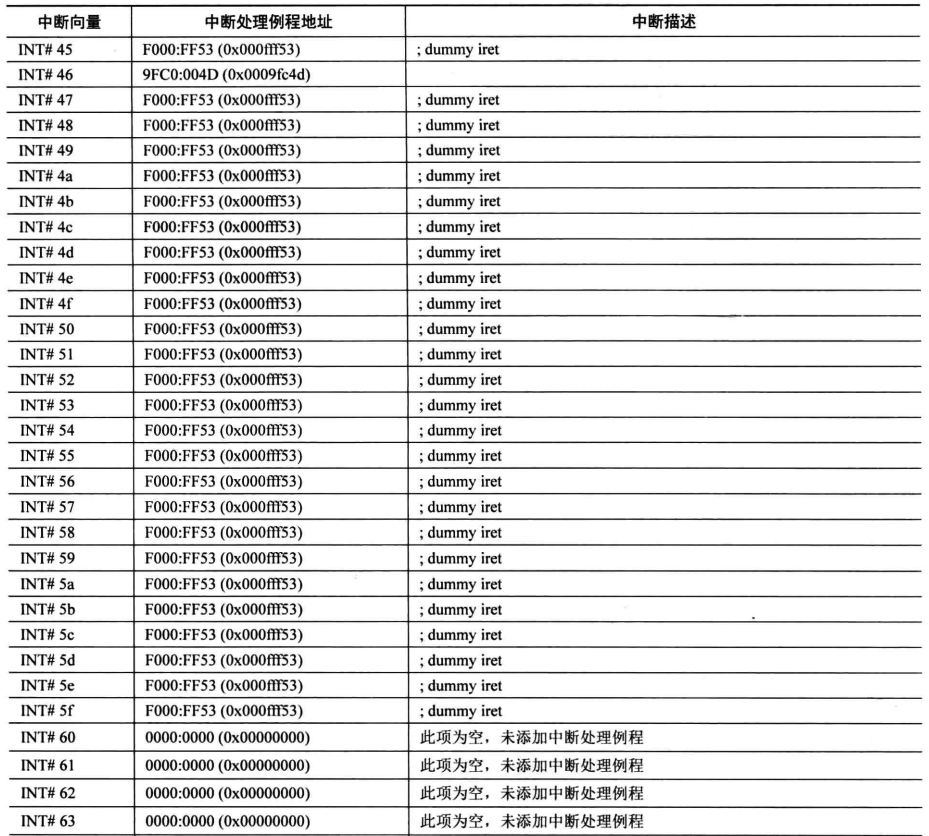
\includegraphics[width=15cm]{中断4}
  \caption{中断向量表4}
  \label{fig:itpt4}
\end{figure}
\begin{figure}[H]
  \centering
  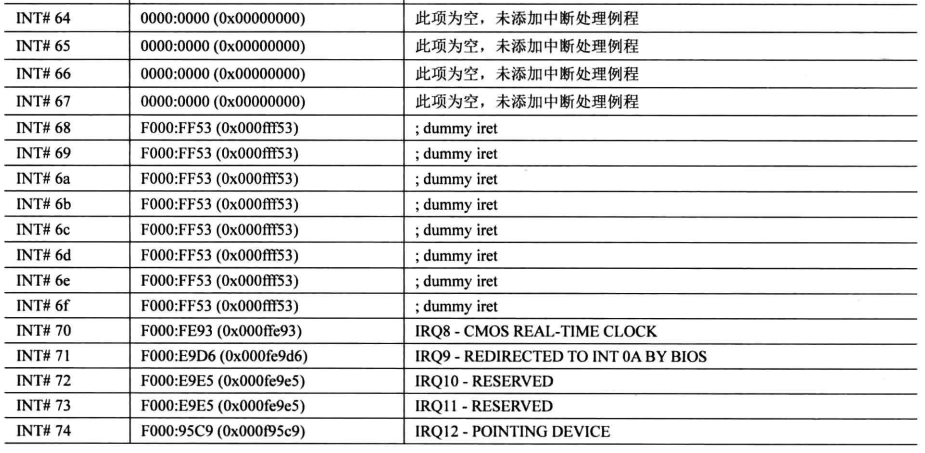
\includegraphics[width=15cm]{中断5}
  \caption{中断向量表5}
  \label{fig:itpt5}
\end{figure}
\begin{figure}[H]
  \centering
  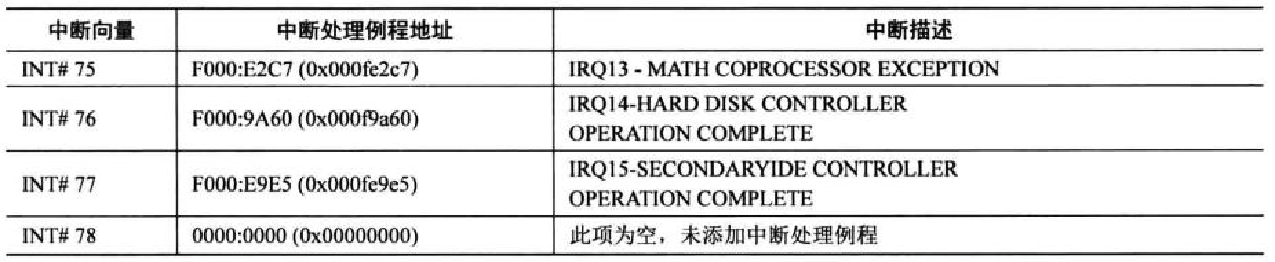
\includegraphics[width=15cm]{中断6}
  \caption{中断向量表6}
  \label{fig:itpt6}
\end{figure}

\section{键盘扫描码}
\label{sec:key}
\begin{figure}[H]
  \centering
  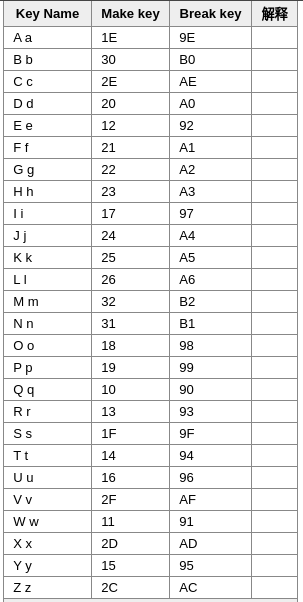
\includegraphics[width=12cm]{扫描码1}
  \caption{Scan code set 1}
  \label{fig:key1}
\end{figure}
\begin{figure}[H]
  \centering
  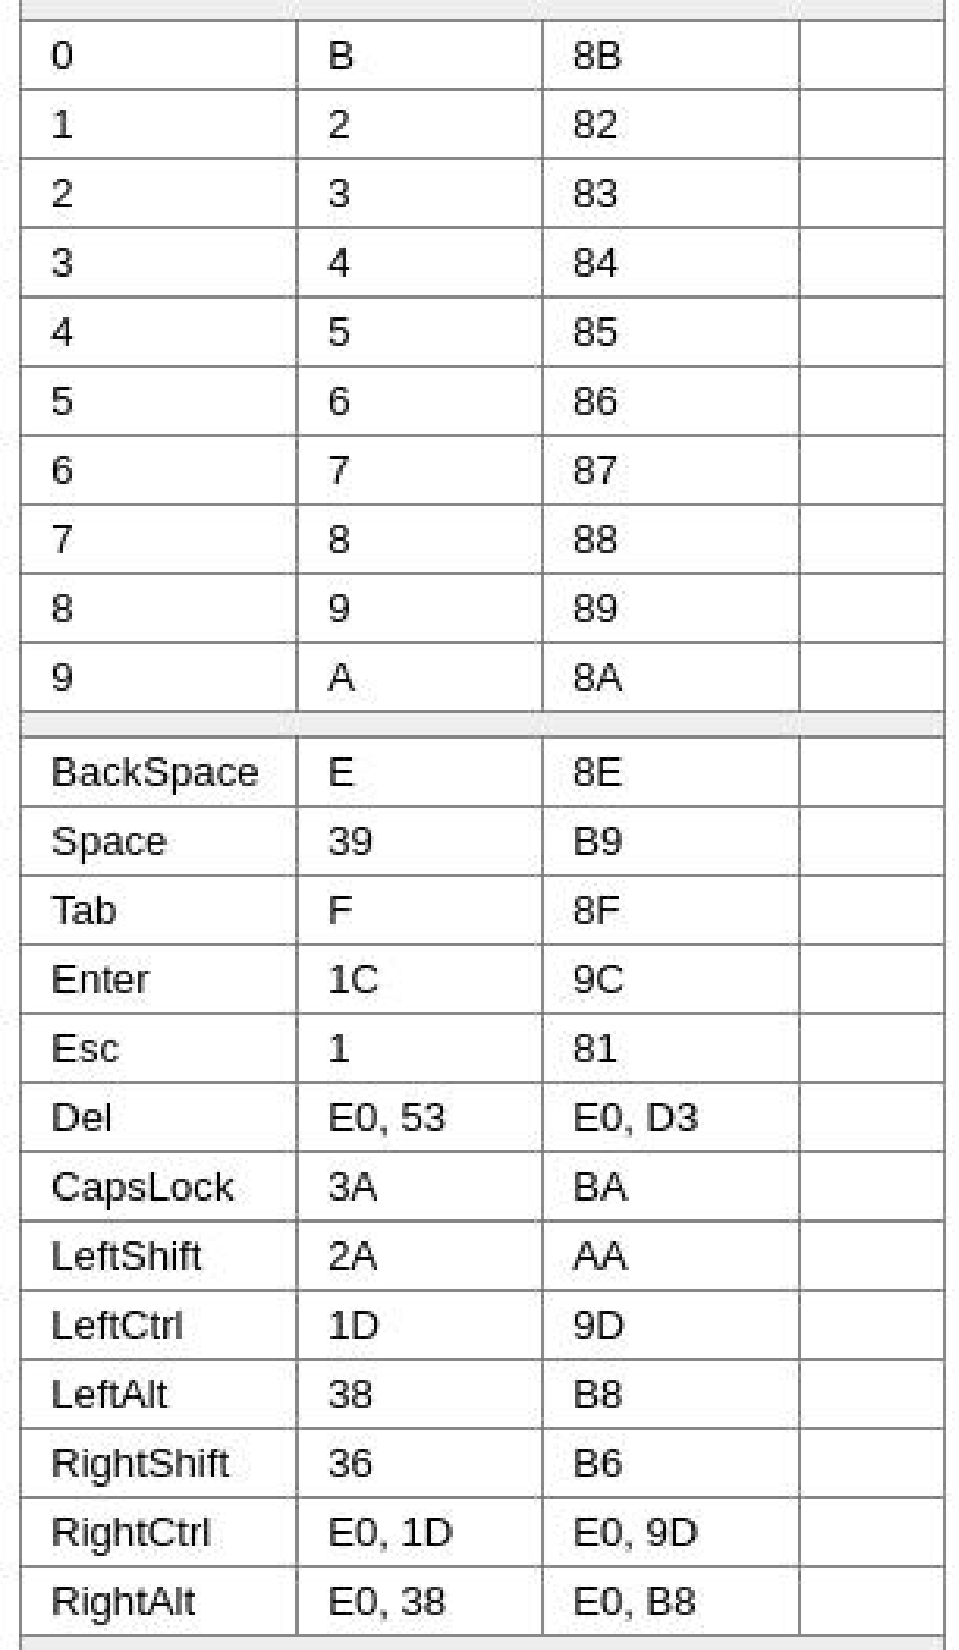
\includegraphics[width=12cm]{扫描码2}
  \caption{Scan code set 1}
  \label{fig:key2}
\end{figure}
\begin{figure}[H]
  \centering
  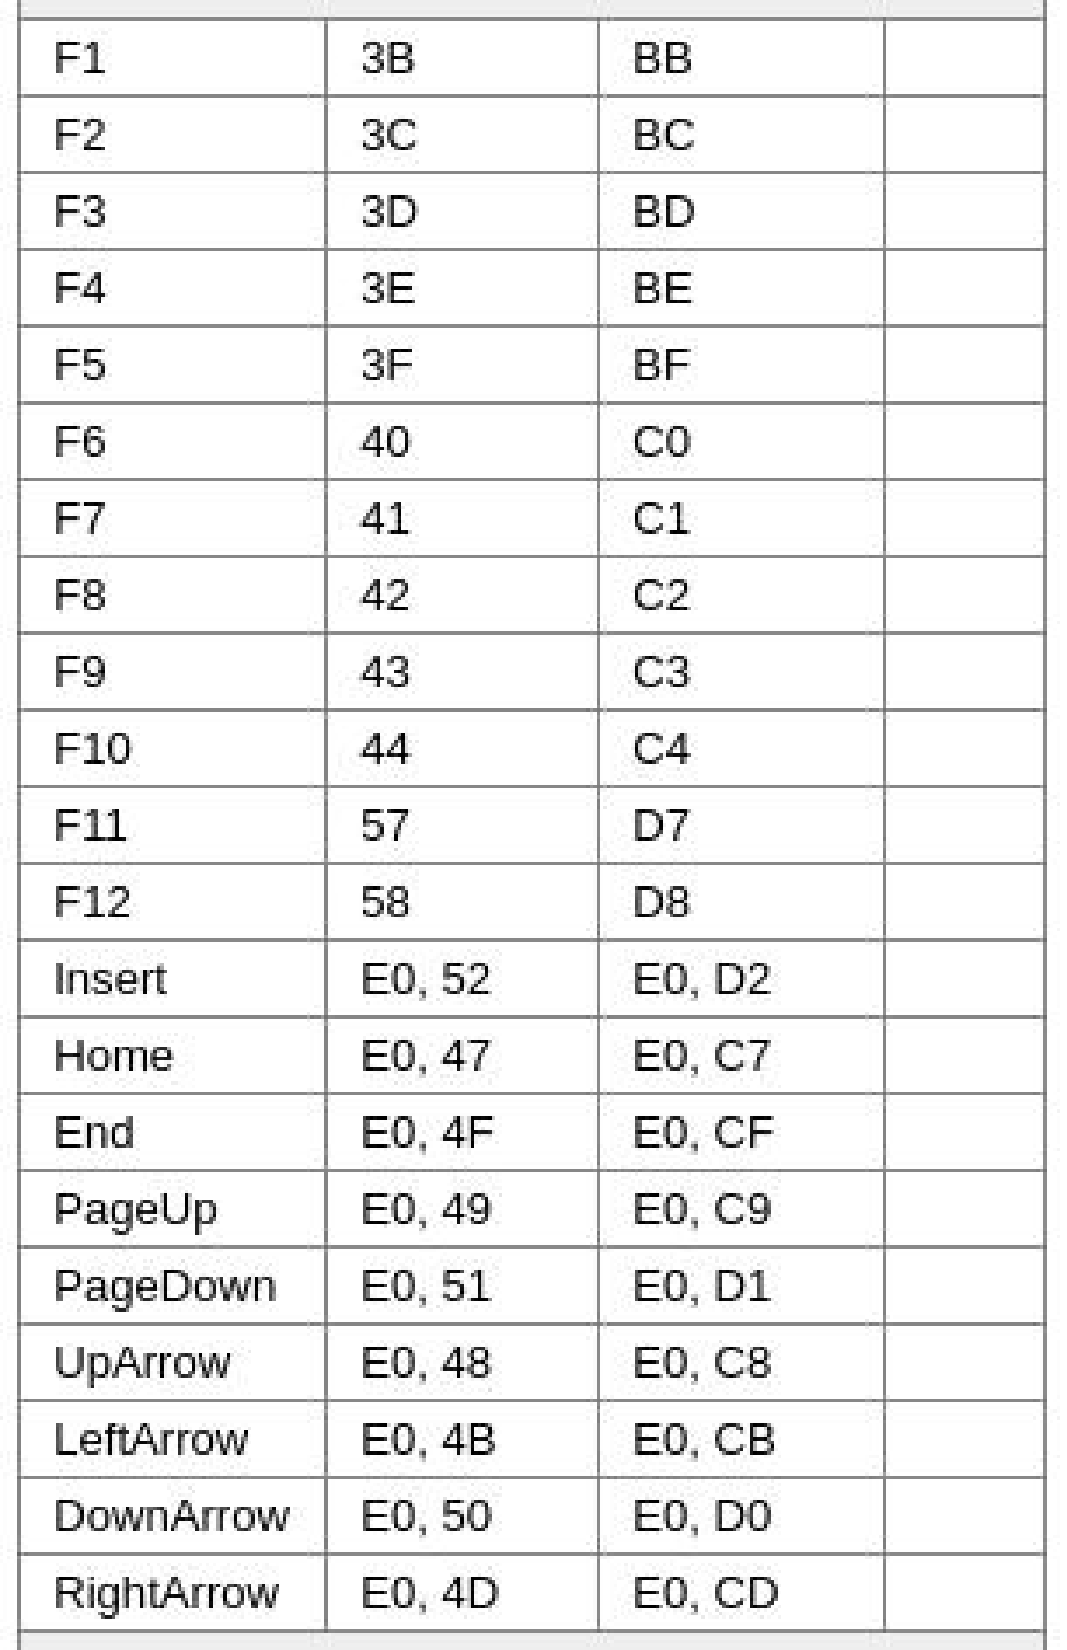
\includegraphics[width=12cm]{扫描码3}
  \caption{Scan code set 1}
  \label{fig:key3}
\end{figure}
\begin{figure}[H]
  \centering
  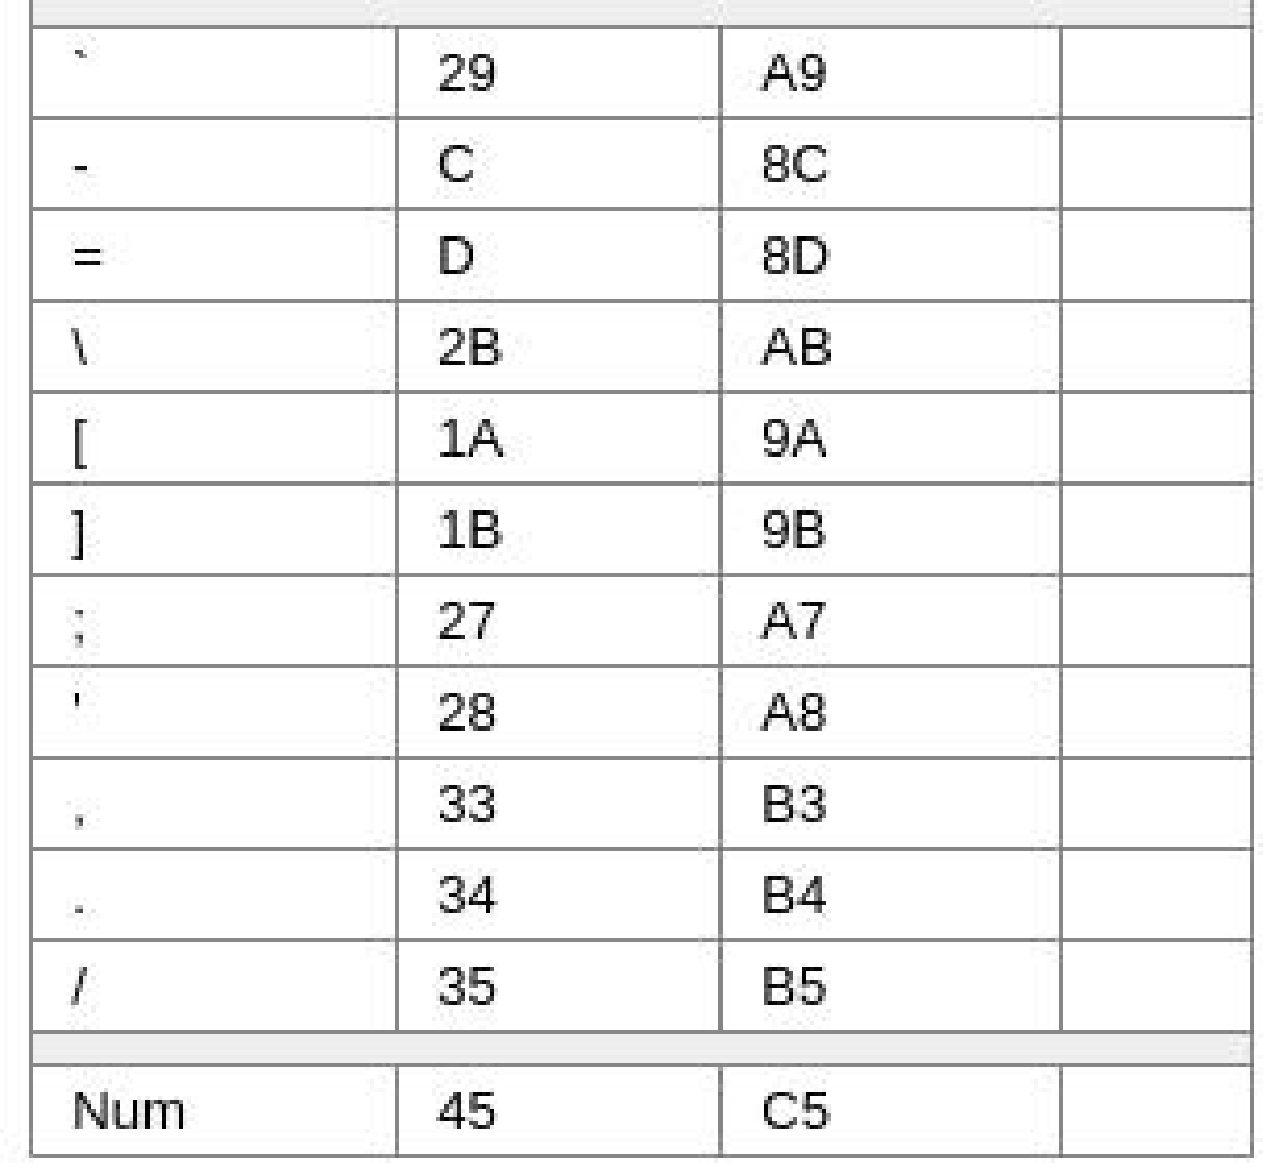
\includegraphics[width=12cm]{扫描码4}
  \caption{Scan code set 1}
  \label{fig:key4}
\end{figure}
%%% Local Variables:
%%% mode: latex
%%% TeX-master: "../thesis"
%%% End:
